% Created 2019-10-03 jue 19:34
% Intended LaTeX compiler: pdflatex
\documentclass[11pt]{article}
\usepackage[utf8]{inputenc}
\usepackage[T1]{fontenc}
\usepackage{graphicx}
\usepackage{grffile}
\usepackage{longtable}
\usepackage{wrapfig}
\usepackage{rotating}
\usepackage[normalem]{ulem}
\usepackage{amsmath}
\usepackage{textcomp}
\usepackage{amssymb}
\usepackage{capt-of}
\usepackage{hyperref}
\usepackage{listings}
\lstalias{ipython}{python}
\lstset{basicstyle=\small\ttfamily, frame=single}
\usepackage{bera}
\author{Invitado}
\date{\today}
\title{Árbol generador de menor costo}
\hypersetup{
 pdfauthor={Invitado},
 pdftitle={Árbol generador de menor costo},
 pdfkeywords={},
 pdfsubject={},
 pdfcreator={Emacs 25.2.2 (Org mode 9.2.3)}, 
 pdflang={English}}
\begin{document}

\maketitle

\section{Problema}
\label{sec:org67aee6c}

Supongamos que a cada arista de la grafica completa \K\textsubscript{n}$\backslash$ se le asigna un valor ("peso").
Si a cada subgráfica le asignamos un peso igual a la suma de los pesos de sus aristas, consideraremos 
el problema de encontrar el árbol generador de menor peso.

\section{Algoritmo de Kruskal}
\label{sec:org665b6ae}

El algoritmo de Kruskal consiste en escoger sucesivamente las aristas más baratas con tal deqno formen
 ciclos con las aristas escogidas previamente.En una gráifca con \(n\) vértices se puede demostrar que
tal algoritmo termina cando hayamos escogido \(n-1\) arrtas, y que el árbol así construido es tal que
tiene costo mínimo.

\section{Implementación}
\label{sec:org906ff51}

Primeramente vamos a importar las bibliotecas que vamos a utilizar 

\lstset{language=ipython,label= ,caption= ,captionpos=b,numbers=none}
\begin{lstlisting}
import networkx as nx
import matplotlib.pyplot as plt
from random import random as random
from scipy.spatial.distance import euclidean
\end{lstlisting}

A continuación definiremos una gráfica aleatoria con 10 vértices

\lstset{language=ipython,label= ,caption= ,captionpos=b,numbers=none}
\begin{lstlisting}
g=nx.gnp_random_graph(10, 0.2)
\end{lstlisting}

Veremos si nuestra gráfica es un bosque.

\lstset{language=ipython,label= ,caption= ,captionpos=b,numbers=none}
\begin{lstlisting}
nx.is_forest(g), nx.is_connected(g)
\end{lstlisting}

\begin{verbatim}
(True, False)
\end{verbatim}

A continuación dibujaremos esta gráfica.

\lstset{language=ipython,label= ,caption= ,captionpos=b,numbers=none}
\begin{lstlisting}
nx.draw(g, with_labels=True)
\end{lstlisting}

\begin{center}
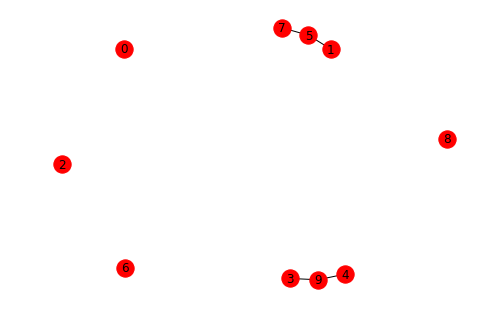
\includegraphics[width=.9\linewidth]{./obipy-resources/2629GNB.png}
\end{center}

Calcularemos las componentes conexas de esta gráfica:

\lstset{language=ipython,label= ,caption= ,captionpos=b,numbers=none}
\begin{lstlisting}
list(nx.connected_components(g))
\end{lstlisting}

\begin{verbatim}
[{0}, {1, 5, 7}, {2}, {3, 4, 9}, {6}, {8}]
\end{verbatim}

Veamos la componente que contiene al vértice 1.

\lstset{language=ipython,label= ,caption= ,captionpos=b,numbers=none}
\begin{lstlisting}
nx.node_connected_component(g, 1)
\end{lstlisting}

\begin{verbatim}
{1, 5, 7}
\end{verbatim}

A continuación dibujaremos un árbol escogido aleatoriamente.

\lstset{language=ipython,label= ,caption= ,captionpos=b,numbers=none}
\begin{lstlisting}
t=nx.random_tree(10)
nx.draw(t, with_labels=True)
\end{lstlisting}

\begin{center}
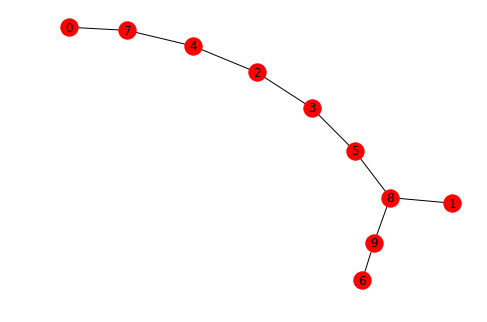
\includegraphics[width=.9\linewidth]{./obipy-resources/2629TXH.png}
\end{center}

\section{Puntos en el plano}
\label{sec:org99d1251}

Si tenemos dos listas de números de tamaño \texttt{n}, podemos dibujar \texttt{n} puntos en el plano,
tomando las coordenadas \texttt{x} de la primera lista y las coordenadas \texttt{y} de la segunda.

\lstset{language=ipython,label= ,caption= ,captionpos=b,numbers=none}
\begin{lstlisting}
plt.plot([1,1,2],[1,2,3],'bx')
plt.axis([0,3,0,4])
plt.show()
\end{lstlisting}

\begin{center}
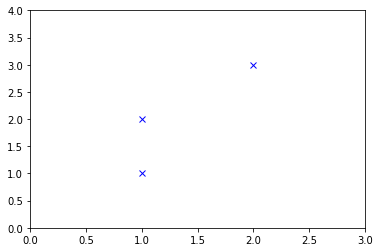
\includegraphics[width=.9\linewidth]{./obipy-resources/2629trT.png}
\end{center}

Vamos a definir una función que dibuje \texttt{n} puntos en el plano aleatoriamente.

\lstset{language=ipython,label= ,caption= ,captionpos=b,numbers=none}
\begin{lstlisting}
def puntos_en_el_plano(n):
    listax=[]
    listay=[]
    for i in range(n):
        listax.append(random())
        listay.append(random())
    return listax, listay
\end{lstlisting}

\lstset{language=ipython,label= ,caption= ,captionpos=b,numbers=none}
\begin{lstlisting}
puntos=puntos_en_el_plano(50)
puntos
\end{lstlisting}

\begin{verbatim}
  ([0.8302879447150826,
  0.060727348191005004,
  0.6906513156041568,
  0.205371949457561,
  0.7831683737299205,
  0.11056422638297958,
  0.011742838736407357,
  0.2961303335734278,
  0.9727979030439259,
  0.5342160128852395,
  0.8481771790742977,
  0.9075572172972087,
  0.5467423958136418,
  0.23578110744199188,
  0.18593011249793323,
  0.41855375976524967,
  0.9032266199908623,
  0.018155445508916235,
  0.1900882959199388,
  0.4271098107250144,
  0.0441816039940196,
  0.5650896364672094,
  0.7800716459908729,
  0.9798234147670897,
  0.5227652041571663,
  0.9852276898842272,
  0.6225250129448031,
  0.6915918087297167,
  0.3105474106963554,
  0.07496578660665076,
  0.27026780525027705,
  0.3732771713342917,
  0.6238570434421412,
  0.5022188085914864,
  0.6927644712586223,
  0.22264210562926645,
  0.6204026084176083,
  0.18199591168750529,
  0.8582757740454406,
  0.5480229017909851,
  0.7016816247948683,
  0.3167595544593431,
  0.3577678595542987,
  0.7394209582847532,
  0.7154456428943944,
  0.7280593044618068,
  0.913929759892807,
  0.857198179271667,
  0.43134465773742314,
  0.7044908779322562],
  [0.03670073151428477,
  0.3880389694745746,
  0.2789738971974399,
  0.24999642162592683,
  0.11799134766518249,
  0.26421242153933266,
  0.7438099494720366,
  0.44942417170652715,
  0.9716963122016856,
  0.5007013336667295,
  0.06340108126682253,
  0.2931651401749381,
  0.9400392356636001,
  0.32673418954545697,
  0.060913772849650716,
  0.057563416622535835,
  0.21113224027263788,
  0.4380323790797218,
  0.24728982278016542,
  0.926669324499162,
  0.3814822958763061,
  0.4412988779588284,
  0.7243734682617066,
  0.4256542615755212,
  0.5817782478620134,
  0.8208066449406247,
  0.6351341340807121,
  0.03164012869633226,
  0.5552027950043776,
  0.4985397196170428,
  0.5346188623691606,
  0.30815951744200376,
  0.12026006444209925,
  0.7535770275801843,
  0.7378331279903371,
  0.5648955655218291,
  0.21620468592821473,
  0.6692482382452427,
  0.6654646234080331,
  0.6510912148159506,
  0.583358076686746,
  0.1939957490774904,
  0.2197351622628343,
  0.9974848898831448,
  0.4787843063398258,
  0.5750518355311282,
  0.622212506124421,
  0.4878799952525623,
  0.5777759205453967,
  0.20952399368695773])
\end{verbatim}

\lstset{language=ipython,label= ,caption= ,captionpos=b,numbers=none}
\begin{lstlisting}
plt.plot(*puntos, 'ro')
plt.show()
\end{lstlisting}

\begin{center}
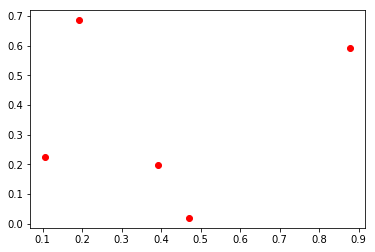
\includegraphics[width=.9\linewidth]{./obipy-resources/2629HAg.png}
\end{center}

Hagamos una función tal que, a partir de dos listas, produzca el dibujo:

\lstset{language=ipython,label= ,caption= ,captionpos=b,numbers=none}
\begin{lstlisting}
def dibujo_puntos(listax, listay):
    plt.plot(listax, listay, 'ro')
    plt.axis([-0.1,1.1,-0.1,1.1])
    plt.gca().set_aspect('equal')
    plt.show()
\end{lstlisting}

\lstset{language=ipython,label= ,caption= ,captionpos=b,numbers=none}
\begin{lstlisting}
dibujo_puntos(*puntos)
\end{lstlisting}

\begin{center}
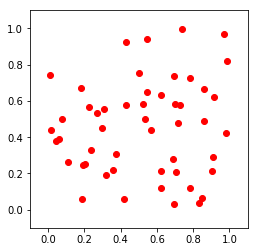
\includegraphics[width=.9\linewidth]{./obipy-resources/2629UKm.png}
\end{center}
\end{document}